\subsection{Analisi delle ridondanze}
\subsubsection{Relazione VALUTAZIONE}
All'interno dello schema ER è stata identificata 1 ridondanza: la relazione valutazione tra le entità alloggio e recensione.\\
Questa ridondanza ci permette di ottenere le recensioni effettuate su un alloggio utilizzando solamente le entità alloggio e recensione.
La sezione della tavola dei volumi di interesse è:

\small
\setlength\extrarowheight{2pt}
\begin{longtable}{|l|c|c|p{6.3cm}|}
      \hline \textbf{Concetto} & \textbf{Tipo} & \textbf{Volume} & \textbf{Motivazione}                                                                                                                         \\\hline
      \endfirsthead

      \hline \textbf{Concetto} & \textbf{Tipo} & \textbf{Volume} & \textbf{Motivazione}                                                                                                                         \\\hline
      \endhead

      % \hline \multicolumn{4}{|r|}{{Continua all pagina successiva}}                                                                                                                                             \\\hline
      \endfoot

      \endlastfoot
      Alloggio                 & E             & 169.000         & {Ipotizziamo che nella piattaforma verranno registrati circa 169 mila alloggi}                                                               \\\hline
      Prenotazione             & E             & 36.000.000      & {Ipotizziamo che sulla piattaforma siano state effettuate circa 36 milioni di prenotazioni}                                                  \\\hline
      Soggiorno                & E             & 34.920.000      & {Ipotizziamo che sulla piattaforma ci siano stati circa 35 milioni di soggiorni}                                                             \\\hline
      Recensione               & E             & 12.000.000      & {Ipotizziamo che sulla piattaforma vengano scritte circa 12 milioni di recensioni}                                                           \\\hline
      Generazione              & R             & 34.920.000      & {Ipotizziamo che sul totale delle prenotazioni, circa il 2\% vengano cancellate. Tutte le altre diventano soggiorni effettivi}               \\\hline
      Correlazione             & R             & 12.000.000      & {Ipotizziamo che circa 1 soggiorno su 6 riceva una recensione da parte dell'utente o dell'host, e che 1 su 6 la riceva da parte di entrambi} \\\hline
      Riserva                  & R             & 36.000.000      & {Ipotizziamo che tutti gli alloggi vengano riservati circa 36 milioni di volte, una volta per ogni prenotazione}                             \\\hline
      Valutazione              & R             & 2.000.000       & {Ipotizziamo che circa 1 recensione su 3 viene scritta verso un alloggio}                                                                    \\\hline
\end{longtable}
\normalsize

\clearpage
\begin{figure}[H]
      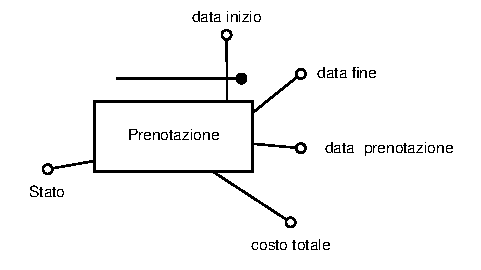
\includegraphics[width=\textwidth]{resources/pdf/page5.pdf}
      \caption{In presenza di ridondanza}
\end{figure}

\begin{figure}[H]
      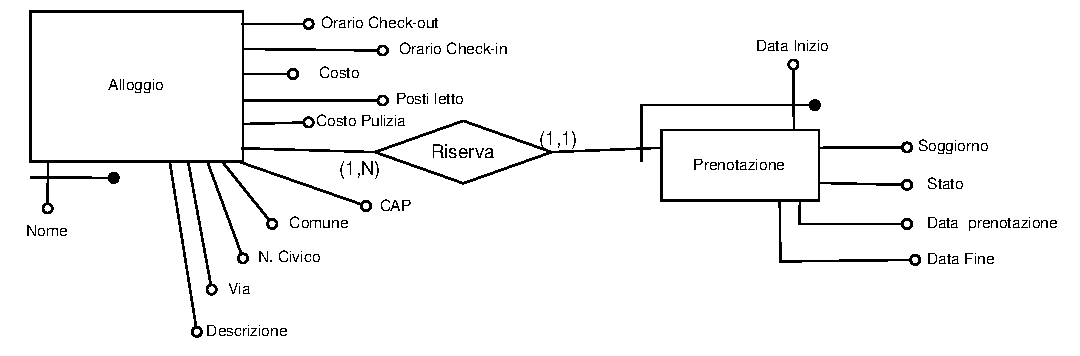
\includegraphics[width=\textwidth]{resources/pdf/page6.pdf}
      \caption{Senza la ridondanza}
\end{figure}

\clearpage
\subsubsection{Tavola degli accessi}
Analizziamo l'operazione "\textbf{Scrittura di una recensione su un alloggio (3000 volte al giorno)}"

\small
\setlength\extrarowheight{2pt}
\begin{longtable}{|lccc|}
      \caption*{In presenza di ridondanza}                                             \\

      \hline \textbf{Concetto} & \textbf{Costrutto} & \textbf{Accessi} & \textbf{Tipo} \\\hline
      \endfirsthead

      \hline \textbf{Concetto} & \textbf{Costrutto} & \textbf{Accessi} & \textbf{Tipo} \\\hline
      \endhead

      \hline \multicolumn{4}{|r|}{{Continua all pagina successiva}}                    \\\hline
      \endfoot

      \hline
      \endlastfoot
      Alloggio                 & E                  & 1                & S             \\%\hline
      Alloggio                 & E                  & 1                & L             \\%\hline
      Recensione               & E                  & 1                & S             \\%\hline
      Valutazione              & R                  & 1                & S             \\%\hline
\end{longtable}
\normalsize

\small
\setlength\extrarowheight{2pt}
\begin{longtable}{|lccc|}
      \caption*{Senza la ridondanza}                                                   \\

      \hline \textbf{Concetto} & \textbf{Costrutto} & \textbf{Accessi} & \textbf{Tipo} \\\hline
      \endfirsthead

      \hline \textbf{Concetto} & \textbf{Costrutto} & \textbf{Accessi} & \textbf{Tipo} \\\hline
      \endhead

      \hline \multicolumn{4}{|r|}{{Continua all pagina successiva}}                    \\\hline
      \endfoot

      \hline
      \endlastfoot
      Alloggio                 & E                  & 1                & L             \\%\hline
      Riserva                  & R                  & 1                & L             \\%\hline
      Prenotazione             & E                  & 1                & L             \\%\hline
      Generazione              & R                  & 1                & L             \\%\hline
      Soggiorno                & E                  & 1                & S             \\%\hline
      Soggiorno                & E                  & 1                & L             \\%\hline
      Correlazione             & R                  & 1                & S             \\%\hline
      Recensione               & E                  & 1                & S             \\%\hline
\end{longtable}
\normalsize


% 
% 
%      TUTTE LE IMMAGINI DI QUESTA PAGINA VANNO MESSE A COPPIE, 2 IMMAGINI PER PAGINA UNA ACCANTO ALL'ALTRA
% 
%

Analisi di complessità in presenza di ridondanza:
\begin{itemize}
      \item In termini di tempo, vengono effettuati un accesso in lettura e tre accessi in scrittura, quindi 3000 + 3000 * 3 * 2 (contiamo doppi gli accessi in scrittura), per un totale di 21 mila accessi.
      \item In termini di spazio, viene aggiunta una relazione in cui si memorizzano i dati chiave dell'alloggio all'interno dell'entità recensione: ipotizziamo quindi 200 byte per ogni recensione scritta.
            Considerando 200 byte per 2.000.000 di recensioni totali, il costo totale in termini di spazio risulta essere 200 * 2.000.000 (~381.47Mb).
\end{itemize}

Analisi di complessità in assenza di ridondanza:
\begin{itemize}
      \item In In termini di spazio, il costo totale è 0 byte.
      \item In termini di tempo, vengono effettuati tre accessi in scrittura e cinque accessi in lettura, quindi 3000 * 5 + 3000 * 3 * 2 (contiamo doppi gli accessi in scrittura), per un totale di 33 mila accessi.
\end{itemize}

Dall'analisi effettuata, con l'assenza di ridondanza, risulta un peggioramento nei tempi di accesso (circa il 35\% di tempo in più) ma un risparmio notevole in termini di spreco di memoria: decidiamo per cui di rimuovere la ridondanza.

\subsection{Eliminazione delle generalizzazioni}
\subsubsection{Entità RECENSIONE}
\begin{figure}[H]
      \centering
      \begin{minipage}[b]{0.45\textwidth}
            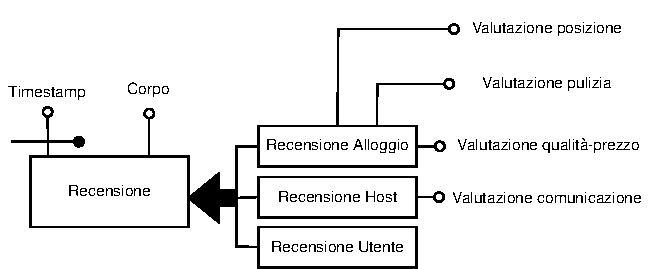
\includegraphics[width=\textwidth]{resources/pdf/page7.pdf}
            \caption{Prima}
      \end{minipage}
      \hfill
      \begin{minipage}[b]{0.45\textwidth}
            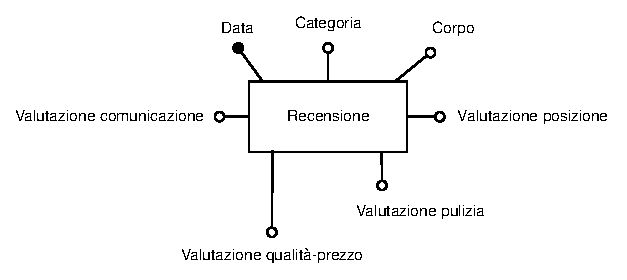
\includegraphics[width=\textwidth]{resources/pdf/page8.pdf}
            \caption{Dopo}
      \end{minipage}
      \caption*{La generalizzazione è di tipo \textbf{totale ed esclusiva}. La decisione consiste nel raggruppamento delle entità	figlie nell'attributo categoria. Gli attributi specifici delle entità figlie (valutazioni) vengono spostate nell'entità padre, diventando annullabili. L'attributo categoria sarà un valore not null.}
\end{figure}

\subsubsection{Entità ALLOGGIO}
\begin{figure}[H]
      \centering
      \begin{minipage}[b]{0.45\textwidth}
            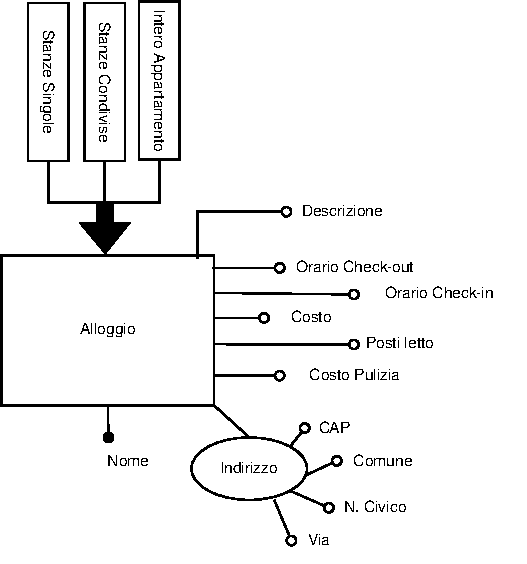
\includegraphics[width=\textwidth]{resources/pdf/page9.pdf}
            \caption{Prima}
      \end{minipage}
      \hfill
      \begin{minipage}[b]{0.45\textwidth}
            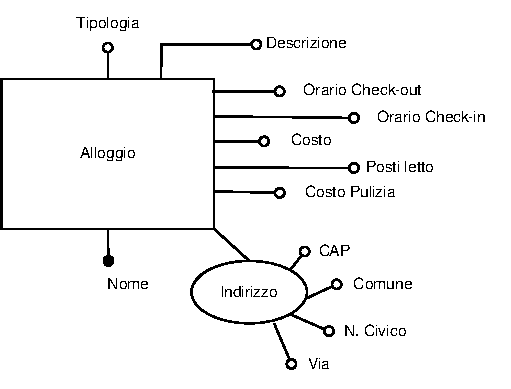
\includegraphics[width=\textwidth]{resources/pdf/page10.pdf}
            \caption{Dopo}
      \end{minipage}
      \caption*{La generalizzazione è di tipo \textbf{totale ed esclusiva}. La decisione consiste nel raggruppamento delle entità	figlie nell'attributo tipologia, con valore not null.}
\end{figure}

\subsubsection{Entità UTENTE}
\begin{figure}[H]
      \centering
      \begin{minipage}[b]{0.45\textwidth}
            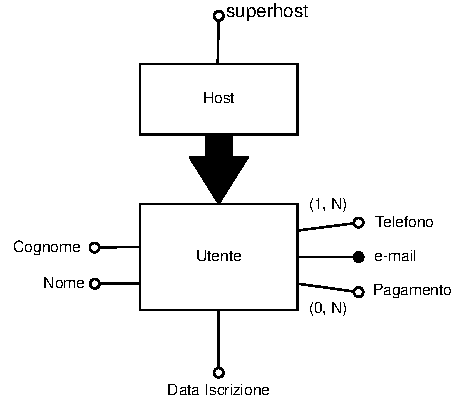
\includegraphics[width=\textwidth]{resources/pdf/page11.pdf}
            \caption{Prima}
      \end{minipage}
      \hfill
      \begin{minipage}[b]{0.45\textwidth}
            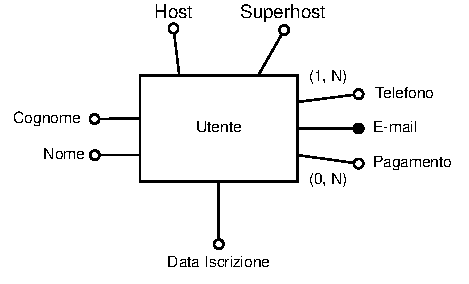
\includegraphics[width=\textwidth]{resources/pdf/page12.pdf}
            \caption{Dopo}
      \end{minipage}
      \caption*{La generalizzazione è di tipo \textbf{totale ed esclusiva}. La decisione consiste nel raggruppamento dell'entità figlia nell'attributo host, con valore not null. L'attributo superhost dell'entità figlia viene trasferito al padre.}
\end{figure}


\subsection{Partizionamento/accorpamento di entità e associazioni}
\subsubsection{Accorpamento Entità PRENOTAZIONE e SOGGIORNO}
\begin{figure}[H]
      \centering
      \begin{minipage}[b]{0.45\textwidth}
            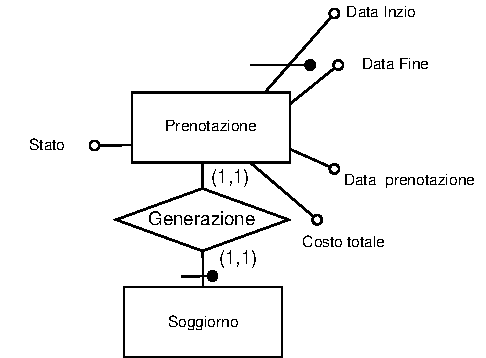
\includegraphics[width=\textwidth]{resources/pdf/page13.pdf}
            \caption{Prima}
      \end{minipage}
      \hfill
      \begin{minipage}[b]{0.45\textwidth}
            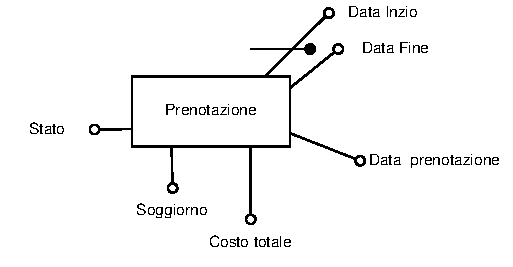
\includegraphics[width=\textwidth]{resources/pdf/page14.pdf}
            \caption{Dopo}
      \end{minipage}
      \caption*{La decisione di accorpare le entità Prenotazione e Soggiorno in un'unica entità con attributo soggiorno (di tipo booleano) deriva dal fatto che l'entità Soggiorno viene generata dalle prenotazioni con stato "confermata".}
\end{figure}

\subsubsection{Partizionamento Entità UTENTE}
\begin{figure}[H]
      \centering
      \begin{minipage}[b]{0.27\textwidth}
            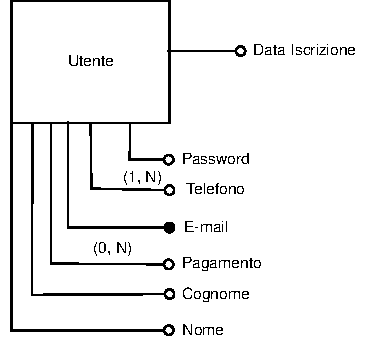
\includegraphics[width=\textwidth]{resources/pdf/page15.pdf}
            \caption{Prima}
      \end{minipage}
      \hfill
      \begin{minipage}[b]{0.63\textwidth}
            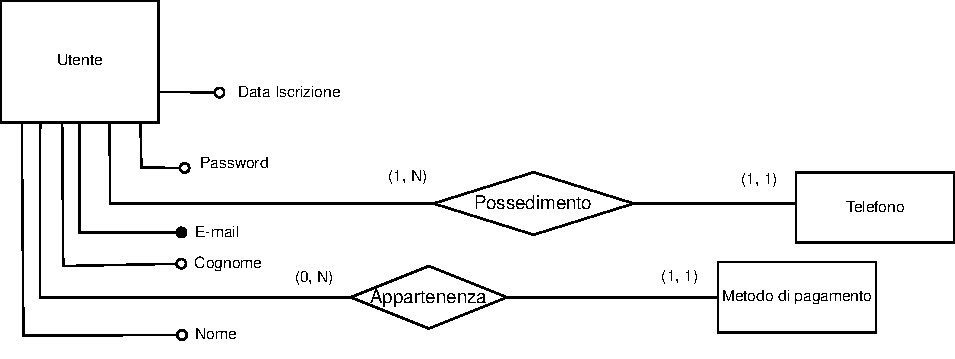
\includegraphics[width=\textwidth]{resources/pdf/page16.pdf}
            \caption{Dopo}
      \end{minipage}
      \caption*{Decidiamo di partizionare l'entità Utente estraendo gli attributi telefono e pagamento, facendoli diventare rispettivamente una nuova entità Telefono, associata a Utente tramite la relazione Possedimento, e una nuova entità Pagamento, associata a Utente tramite la relazione Appartenenza.}
\end{figure}

\begin{figure}[H]
      \centering
      \begin{minipage}[b]{0.40\textwidth}
            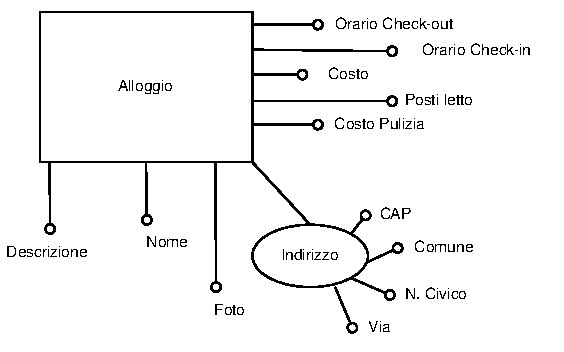
\includegraphics[width=\textwidth]{resources/pdf/page17.pdf}
            \caption{Prima}
      \end{minipage}
      \hfill
      \begin{minipage}[b]{0.50\textwidth}
            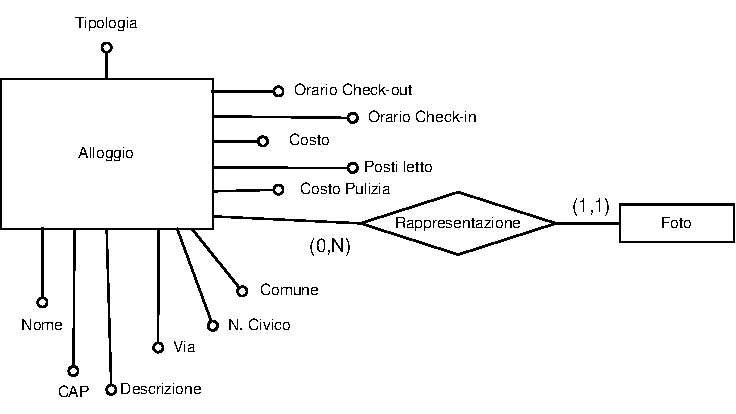
\includegraphics[width=\textwidth]{resources/pdf/page18.pdf}
            \caption{Dopo}
      \end{minipage}
      \caption*{Decidiamo di partizionare ulteriormente l'entità Utente estraendo l'attributo foto, facendolo diventare una nuova entità Foto, associata a Utente tramite la relazione Rappresentazione.}
\end{figure}

\subsection{Eliminazione degli attributi composti}
L’attributo composto “\textbf{indirizzo}” viene eliminato, considerando i suoi componenti come attributi semplici. Nel caso di indirizzo abbiamo: via, numero civico, cap e comune.
Tale eliminazione viene effettuato nell'entità Alloggio